\documentclass{coupled}

\usepackage{graphicx}
\usepackage{amsmath}
\usepackage{amsfonts}
\usepackage{amssymb}

\title{INSTRUCTIONS TO PREPARE A FULL PAPER FOR THE V INTERNATIONAL CONFERENCE ON COMPUTATIONAL METHODS
FOR COUPLED PROBLEMS IN SCIENCE AND ENGINEERING -- COUPLED PROBLEMS 2013}

\author{FIRST A. AUTHOR$^{*}$, SECOND B. AUTHOR$^{\dag}$ AND THIRD C. COAUTHOR$^{\dag}$}

\heading{First A. Author, Second B. Author and Third C. Coauthor}

\address{$^{*}$International Center for Numerical Methods in Engineering (CIMNE)\\
Universidad Polit\'{e}cnica de Catalu\~{n}a\\
Campus Norte UPC, 08034 Barcelona, Spain\\
e-mail: congress@cimne.upc.edu, web page: http://www.cimne.com/
\and
$^{\dag}$Spanish Association for Numerical Methods in Engineering (SEMNI)\\
Edificio C1, Campus Norte UPC\\
Gran Capit\'{a}n s/n, 08034 Barcelona, Spain\\
e-mail: semni@cimne.upc.edu - Web page: http://www.semni.org}

\keywords{Instructions, Coupled Problems, Multiphysics Problems, Applications, Computing Methods}

\abstract{This document provides information and instructions for
preparing a Full Paper to be included in the Proceedings
of {\it Coupled Problems 2013 Conference}. }

\begin{document}
%\maketitle

\section{INTRODUCTION}

All the participants whose Abstract has been accepted for presentation at the Conference are kindly requested to submit the Full Paper electronically via the web page of the Conference, http://congress.cimne.com/coupled2013 \emph{before  February 28}, 2013. {\it The submission of the full paper is not mandatory but highly recommended as the Conference Proceedings (full papers) will be submitted for indexation in the Conference Proceedings Citation Index - ISI Web of Knowledge (Thomson Reuters) and SCOPUS database}. The Full Paper should be written following the format of macros for submission. The file must be converted to  Portable Document Format (PDF) before submission via the Conference site. The organizers do not commit themselves to include in the Proceedings any Full Paper received later than the above-mentioned deadline. The corresponding author should be the speaker, and is expected to register and pay his registration fee during the advance period (before 28 February 2013) for the Full Paper to be included in the technical program of the Conference.

\section{GENERAL ESPECIFICATIONS}

The Full Paper must be written in English within a printing box of 16cm x 21cm, centered in the page. The Full Paper including figures, tables and references must have a minimum length of 6 pages and must not exceed 12 pages. Maximum file size is 4 MB.

\section{TITLE, AUTHORS, AFFILIATION, KEY WORDS}

The first page must contain the Title, Author(s), Affiliation(s),
Key words and the Summary. The Introduction must begin immediately
below, following the format of this template.

\subsection{Title}

The title should be written centered, in 14pt, boldface Roman, all
capital letters. It should be single spaced if the title is more
than one line long.

\subsection{Author}

The author's name should include first name, middle initial and
surname. It should be written centered, in 12pt boldface Roman,
12pt below the title.

\subsection{Affiliation}

Author's affiliation should be written centered, in 11pt Roman,
12pt below the list of authors. A 12pt space should separate two
different affiliations.

\subsection{Key words}

Please, write no more than six key words. They should be written
left aligned, in 12pt Roman, and the line must begin with the
words {\bf Key words}: boldfaced. A 12pt space should separate the
key words from the affiliations.

\subsection {Summary (optional)}

Use 12pt Italic Roman for the summary. The word {\bf Summary} must
be set in boldface, not italicized, at the beginning of the first
line. The text should be justified and separated 12pt from the key
words, as shown in the first page of these instructions.

\section{HEADINGS}

\subsection{Main headings}

The main headings should be written left aligned, in 12pt,
boldface and all capital Roman letters. There should be a 12pt
space before and 6pt after the main headings.

\subsection {Secondary headings}

Secondary headings should be written left aligned, 12 pt, boldface
Roman, with an initial capital for first word only. There should
be a 12pt space before and 6pt after the secondary headings.

\section{EDITORIAL HEADING}

The first page has to include the Editorial Heading, as shown in
the first page of these instructions. Successive pages will
include the name of the authors.

\section{TEXT}

The normal text should be written single-spaced, justified, using
12pt (Times New) Roman in one column. The first line of each
paragraph must be indented 0.5cm. There is not inter-paragraph
spacing.

\section{PAGE NUMBERS}

In order to organize the Full Paper, it is better to number
the pages. Page numbers are not included in the printing box.

\section{FIGURES}

All figures should be numbered consecutively and captioned. The
caption title should be written centered, in 10pt Roman, with
upper and lower case letters.

\begin{figure}[t]
\centering
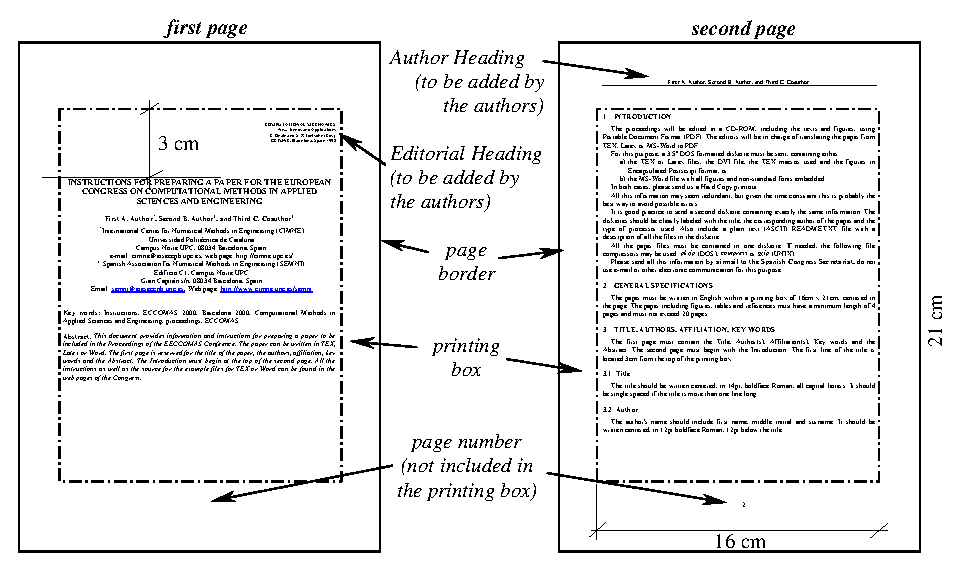
\includegraphics[width=11cm]{firstpage}
\caption{Page layout}
\end{figure}

A 6pt space should separate the figure from the caption, and a
12pt space should separate the upper part of the figure and the
bottom of the caption from the surrounding text.

Figures may be included in the text or added at the bottom of the paper.

\section{EQUATIONS}

A displayed equation is numbered, using Arabic numbers in
parentheses. It should be centered, leaving a 6pt space above and
below to separate it from the surrounding text.

The following example is a single line equation:
\vskip-.6cm
\begin{eqnarray}
Ax = b
\end{eqnarray}

The next example is a multi-line equation:
\vskip-.6cm
\begin{eqnarray}
Ax = b \\
Ax = b \nonumber
\end{eqnarray}

\section{TABLES}

All tables should be numbered consecutively and captioned, the
caption should be 10pt Roman, upper and lower case letters.

\begin{table}[h!]
\caption{Example of the construction of one table}
\begin{center}
\begin{tabular}{*{3}{c}}
\hline
C11 & C12 & C13 \\
\hline
C21 & C22 & C23 \\
\hline
C31 & C32 & C33 \\
\hline
C41 & C42 & C43 \\
\hline
C51 & C52 & C53 \\
\hline
\end{tabular}
\end{center}
\end{table}

A 6pt space should separate the table from the caption, and a 12pt
space should separate the table from the surrounding text.

\section{FORMAT OF REFERENCES}

References should be quoted in the text by superscript
numbers \cite{Zienkiewicz,Idelsohn} and grouped together at the end of the Full Paper in numerical order as shown in these instructions.

\section{CONCLUSIONS}

\begin{itemize}
\item[-] Full Papers in format for publication should be submitted electronically via the web page of the Conference http://congress.cimne.com/coupled2013, before February 28th 2013. They must be converted to  Portable Document Format (PDF) before submission. The maximum size of the file is 4 Mb.

\item[-] The speaker (corresponding author) is expected to pay his registration fee during the advance period (before February 28th 2013) for the presentation to be included in the final program of the Conference. Only one presentation per registration is allowed.
\end{itemize}

\begin{thebibliography}{99}
\bibitem{Zienkiewicz}  Zienkiewicz, O.C. and  Taylor, R.L. \textit{The finite element method}. McGraw Hill,
Vol. I., (1989), Vol. II., (1991).
\bibitem{Idelsohn} Idelsohn, S.R. and O\~{n}ate, E. Finite element and finite volumes. Two good friends.
\textit{Int. J. Num. Meth. Engng.} (1994) \textbf{37}:3323--3341.
\end{thebibliography}

\end{document}


